%----------------------------------------------------------------------
\section{Future Work}
%----------------------------------------------------------------------
Online adaptive

The system we have implemented is offline. It can be turned into online adaptive one by keeping a sliding window of previous workloads. 

Schema graph to data graph

Our system currently supports SPARQL like queries over schema graph instead of data graph. It could be further improved to support queries over data graph without changing the high-level solution framework. The key part that needs to be modified is to label each unique node and take isomorphism into consideration during query decomposition.  

Better Cube-Planner and Structure-Planner

We used greedy approach for ranking cuboids and substructures. Although it worked well in our experiment. But greedy approach is not holistic enough. For instance???

Multi-Thread

The system can be made multi-thread so that joining work of queries could be done when the system is waiting for graph database’s query execution. 

%----------------------------------------------------------------------
\section{Reflection on Neo4j}
%----------------------------------------------------------------------
%----------------------------------------------------------------------
\subsection{Aggregation Size Estimation}
%----------------------------------------------------------------------
We found that Neo4j has a very coarse way of estimating result size of aggregation queries. It simply takes square root of table size before aggregation, without regards to aggregation attributes. Of course this will lead to a huge bias. 

For instance, let’s look at the following 2 queries with the same structure:

(1) match (u:User)-[]-(b:Badge)  match (u:User)-[]-(p:Post)  match (p:Post)-[]-(t:Tag)  return  t.TagName, count(*)

\begin {figure}[H]
\centering
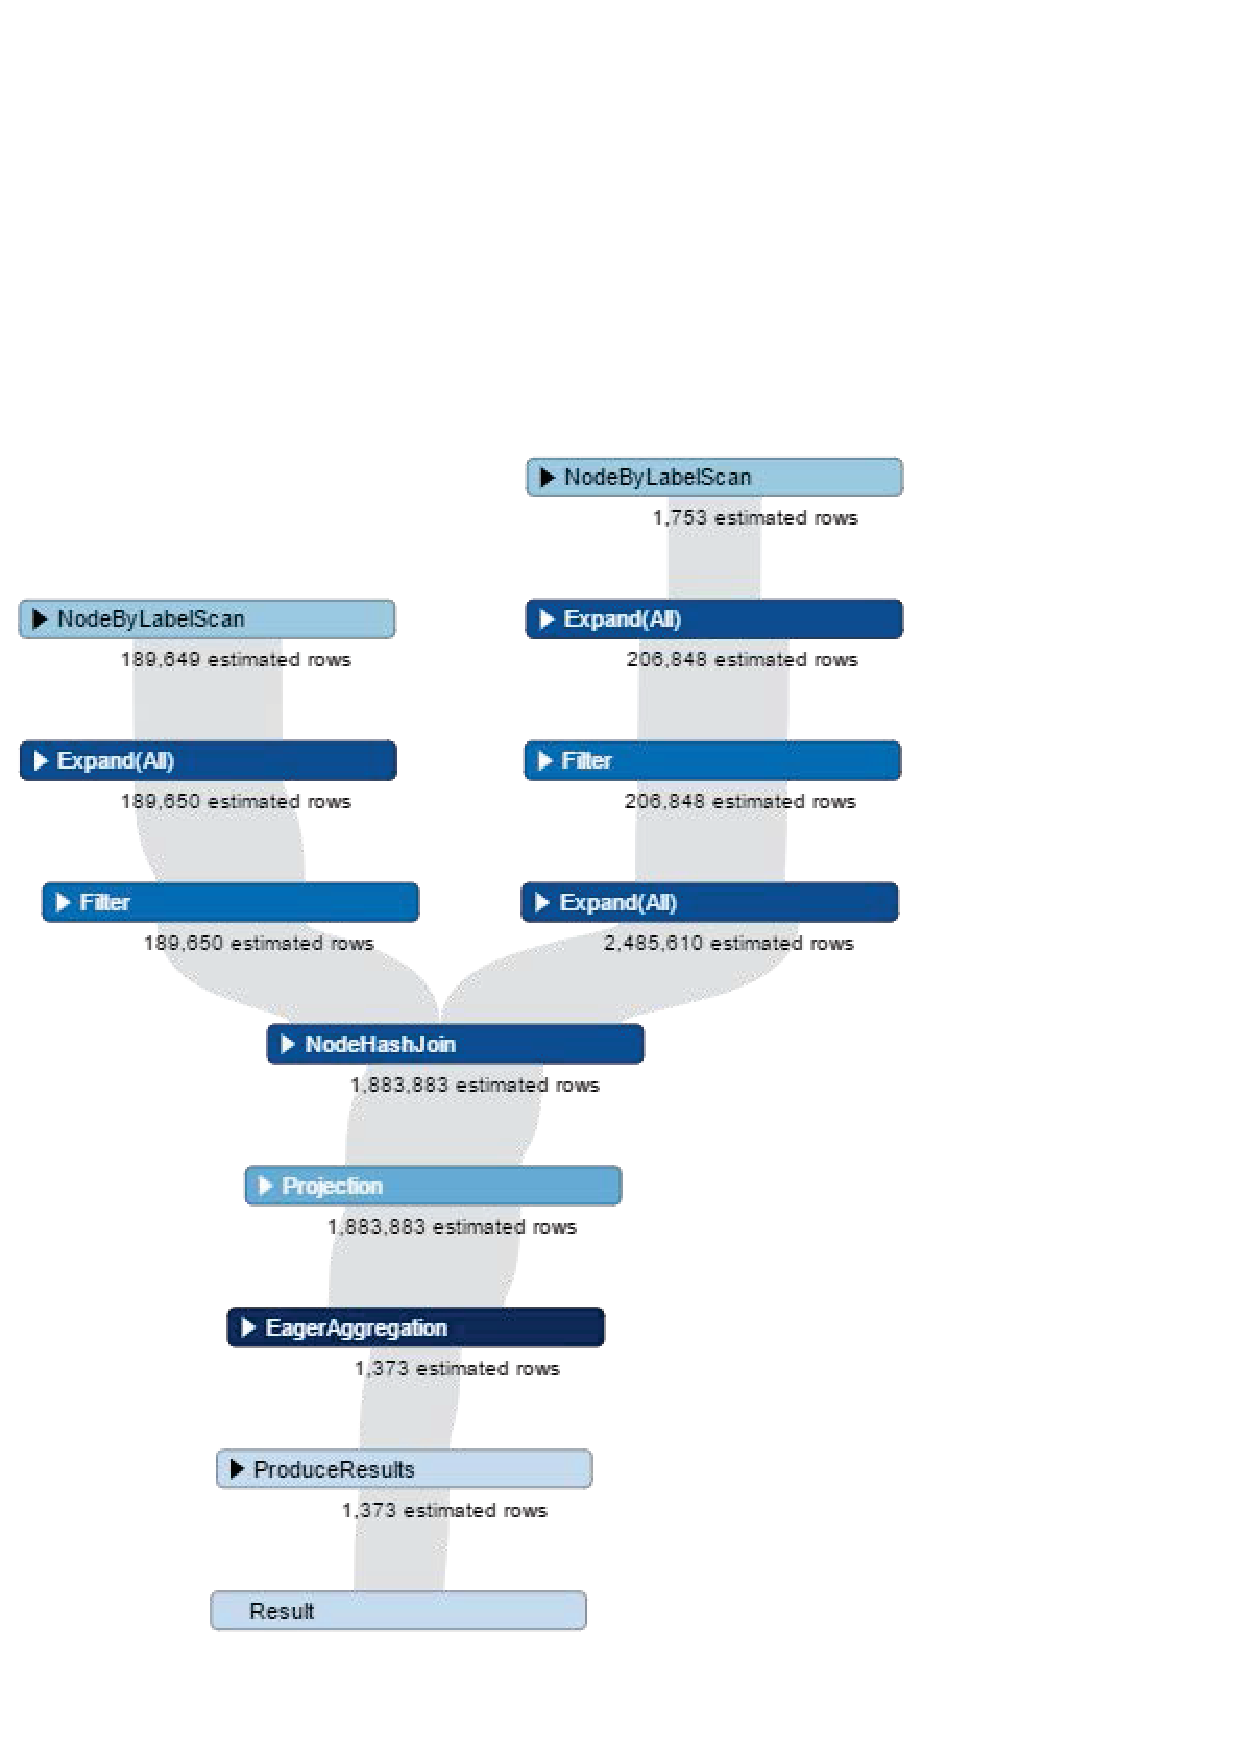
\includegraphics[scale=0.6]{pic/61.png}
\end{figure}

(2) match (u:User)-[]-(b:Badge)  match (u:User)-[]-(p:Post)  match (p:Post)-[]-(t:Tag)  return  t.TagName, id(u), id(b), id(p), count(*)

\begin {figure}[H]
\centering
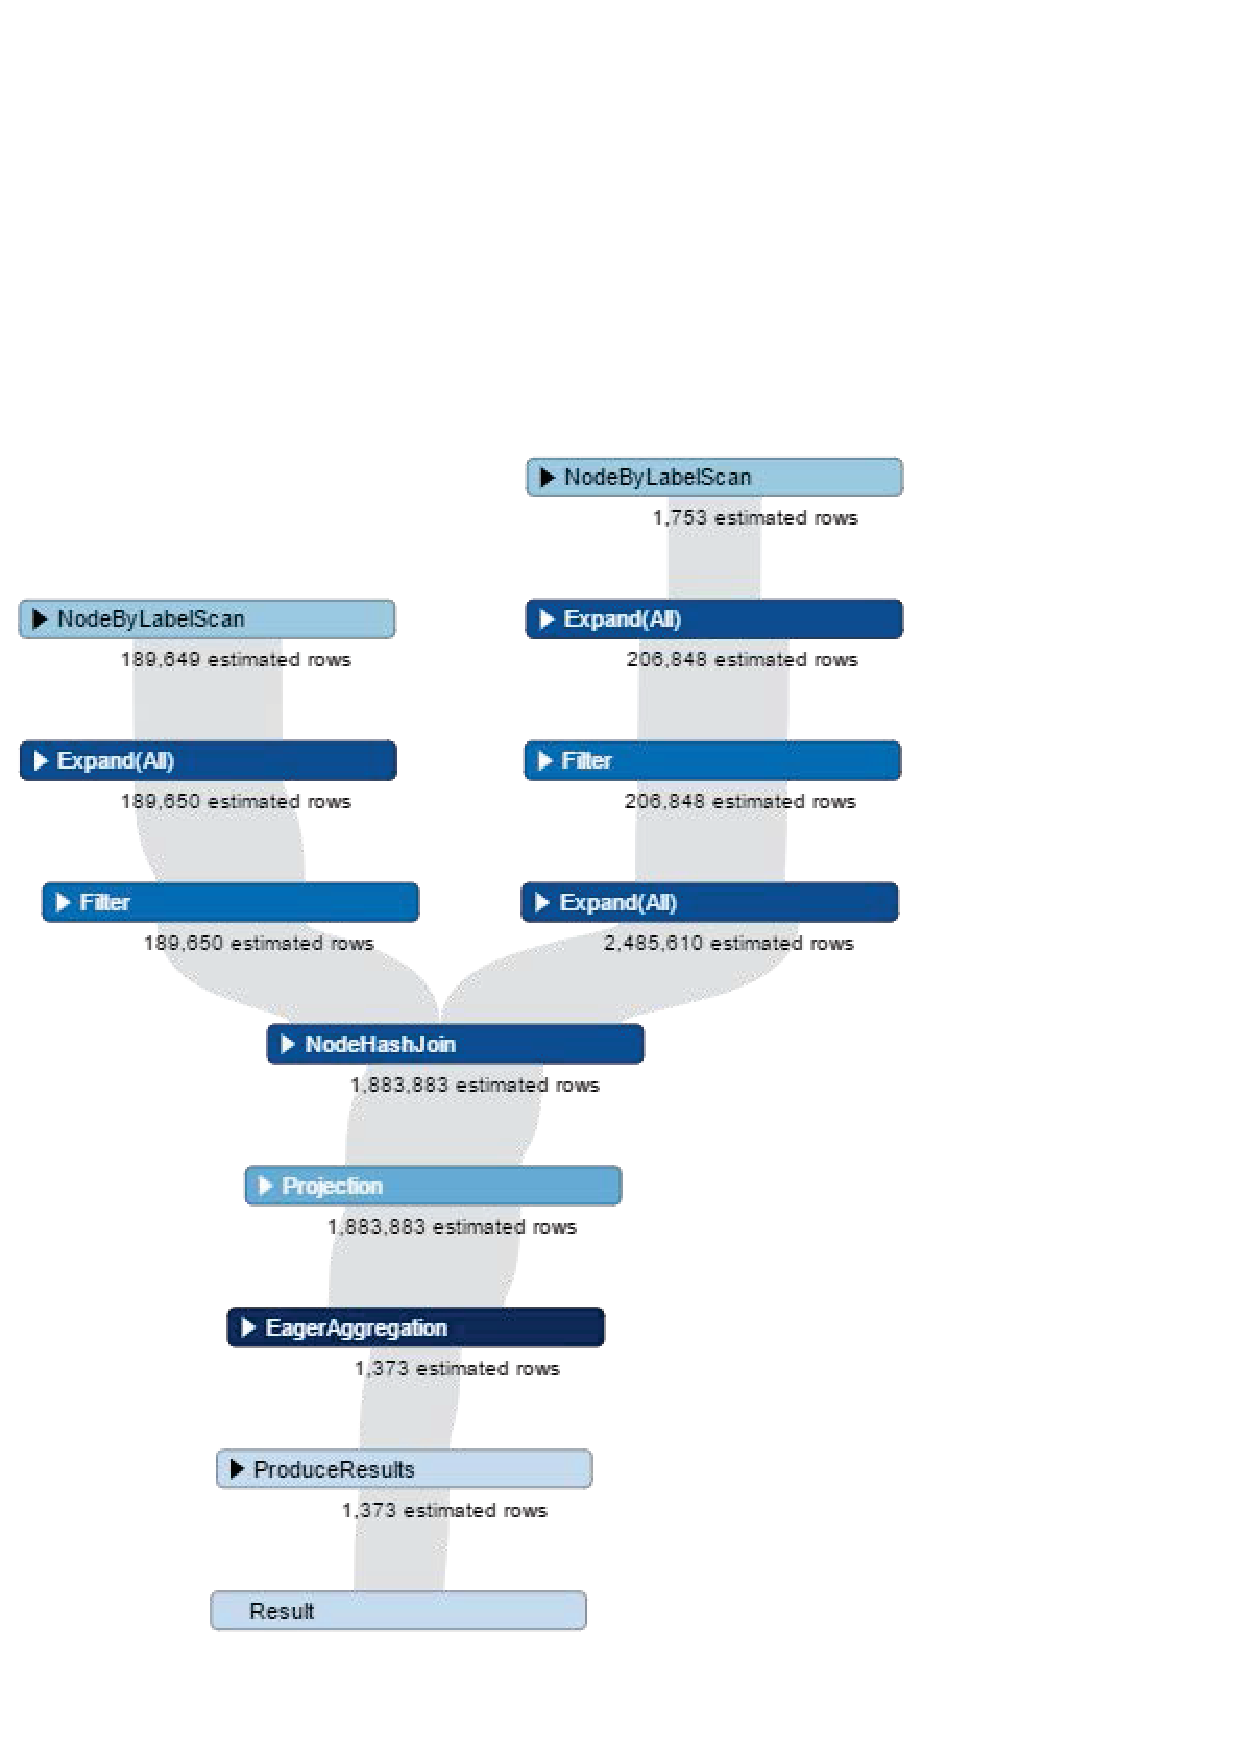
\includegraphics[scale=0.6]{pic/61.png}
\end{figure}

Since (2) contains ids of all queried nodes(User, Badge and Post), supposedly (2) should have a much larger result size than (1). However in Neo4j will estimate that (1) and (2) have the same result size. 

Therefore in our implementation we use the following function to predict cuboid size:
Cuiboid(att_1, att_2… att_n)= Product of(|att_i|) * (shrinking factor)^(n-1)
